\renewcommand{\nomebreve}{block\_diag\_mat}
\renewcommand{\titolo}{Detecting blocks in a matrix}

\introduzione{}

\noindent
A \emph{diagonal matrix} is a square matrix all of whose off-diagonal elements are zeros. A \emph{block diagonal matrix} is a square block matrix all of whose main-diagonal blocks are square matrices and all off-diagonal blocks are zero matrices.  That is, a block diagonal matrix $\mathbf{A}$ has the form

\begin{figure}[!h]
\[
\mathbf{A} = \begin{bmatrix} 
  \mathbf{A}_1 & \mathbf{0}    & \cdots & \mathbf{0}   \\
  \mathbf{0}   & \mathbf{A}_2  & \cdots & \mathbf{0}   \\
  \vdots       & \vdots        & \ddots & \vdots       \\
  \mathbf{0}   & \mathbf{0}    & \cdots & \mathbf{A}_n
\end{bmatrix}
\]
  \label{fig:block_structure}
  \caption{the block structure of a block diagonal matrix}
\end{figure}

where $\mathbf{A}_k$ is a square matrix for all $k = 1, \ldots, n$.
The picture might help clarifying the concept.
\begin{table}[!h]
  \begin{minipage}{.5\textwidth}
    \centering
    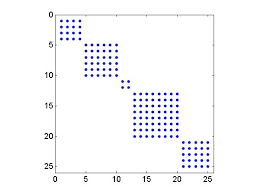
\includegraphics[width=0.60\textwidth]{figures/block_diag_mat_gen_example.png}\\
    {\bf see:} the structure of a block diagonal matrix
  \end{minipage}%
  \begin{minipage}{.5\textwidth}
    \centering
    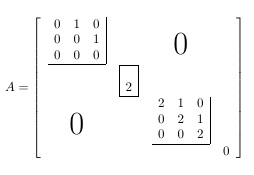
\includegraphics[width=0.60\textwidth]{figures/block_diag_mat_one_example_with_structure_highlighted.png}\\
    {\bf note:} also the entries within the diagonal blocks might be zero
    \end{minipage}
%}      
\end{table}

A matrix can be considered as a block diagonal matrix with only one block if and only if it is square. However, our ambition is to read the structure of a given square matrix as to detect as many blocks as possible. An $n\times n$ matrix can be considered as a block diagonal matrix with $n$ blocks if and only if it is a diagonal matrix.

We generalize this notion of decomposing a given matrix into blocks to general rectangualar matrices.
The block structure to be read remains a square matrix whose off-diagonal blocks are zero matrices, as in Figure~\ref{fig:block_structure}, but now the diagonal elements are arbitrary (possibly non-square) blocks of the input matrix. Under these constraints, the maximum number of blocks in which we can decompose the following matrix is $4$.

\begin{table}[!h]
  \begin{minipage}{.5\textwidth}
    \centering
\[
\left(
\begin{array}{cccccc|ccccc}
    1 & 0 & 3  & 0 & 0 & 0   &  0 & 0 & 0 & 0  & 0     \\
    0 & 0 & 0  & 2 & 1 & 5   &  0 & 0 & 0 & 0  & 0     \\   \hline
    0 & 0 & 0  & 0 & 0 & 0   &  6 & 0 & 0 & 0  & 0     \\
    0 & 0 & 0  & 0 & 0 & 0   &  7 & 0 & 0 & 0  & 0     \\
    0 & 0 & 0  & 0 & 0 & 0   &  2 & 0 & 5 & 0  & 0     \\
    0 & 0 & 0  & 0 & 0 & 0   &  0 & 0 & 3 & 2  & 0     \\
    0 & 0 & 0  & 0 & 0 & 0   &  0 & 0 & 0 & 0  & 2     \\
\end{array}\right)
\]
    {\bf sub-optimal read:} 2 blocks
  \end{minipage}%
  \begin{minipage}{.5\textwidth}
    \centering
\[
\left(
\begin{array}{ccc|ccc|cccc|c}
    1 & 0 & 3  & 0 & 0 & 0   &  0 & 0 & 0 & 0  & 0     \\   \hline
    0 & 0 & 0  & 2 & 1 & 5   &  0 & 0 & 0 & 0  & 0     \\   \hline
    0 & 0 & 0  & 0 & 0 & 0   &  6 & 0 & 0 & 0  & 0     \\
    0 & 0 & 0  & 0 & 0 & 0   &  7 & 0 & 0 & 0  & 0     \\
    0 & 0 & 0  & 0 & 0 & 0   &  2 & 0 & 5 & 0  & 0     \\
    0 & 0 & 0  & 0 & 0 & 0   &  0 & 0 & 3 & 2  & 0     \\   \hline
    0 & 0 & 0  & 0 & 0 & 0   &  0 & 0 & 0 & 0  & 2     \\
\end{array}\right)
\]
    {\bf optimal read:} 4 block
    \end{minipage}
%} 
\end{table}

Vogliamo valutare e consentire l'espressione delle seguenti competenze:
\begin{description}
\item[subtask di tipo~$t=1$] saper identificare quali archi siano dei bridge;
\item[subtask di tipo~$t=2$] saper identificare quali nodi siano dei cutnode;
\item[subtask di tipo~$t=3$] specificare per ogni nodo $v$ quante siano le componenti connesse del grafo ottenuto da $G$ per rimozione del nodo $v$. Se intendi fornire una soluzione lineare anche per questo tipo di subtask allora potrebbe convenirti acquisire la nozione di componente biconnessa esposte nella sezione di appendice. 
\end{description}


\sezionetesto{Input ed Output}

Input ed output avvengono da \verb'stdin' e su \verb'stdout' rispettivamente.
La prima riga dell'input contiene i tre numeri $t$, $n$ ed $m$, nell'ordine e separati da spazio. Il numero $t$ indica la richiesta come da tabella sopra, mentre $n:=|V|$ e $m:=|E|$. Per rappresentare $G$, i nodi in $V$ sono messi in corrispondenza biunivoca coi numeri naturali da~$0$ a~$n-1$.
Seguono $m$ righe dove ciascuna riga codifica un diverso arco $e=uv\in E$ riportandone gli estremi. In pratica, dove assumiamo $u < v$, la riga contiene i due numeri $u$ e $v$, nell'ordine, e separati da spazio.
Queste $m$ righe sono date in ordine lessicografico (si vedano gli esempi).

\indent
Per subtask di tipo $t=1$ l'output consta di $m$ cifre binarie stampate una per riga. L'$i$-esima di queste cifre è $1$ se l'$i$-esimo arco letto in input è un bridge di $G$, altrimenti è $0$.\\
\indent
Per subtask di tipo $t=2$ l'output consta di $n$ cifre binarie stampate una per riga. L'$i$-esima di queste cifre è $1$ se il nodo $(i-1)$ è un cutnode di $G$, altrimenti è $0$.\\
\indent
Per subtask di tipo $t=3$ l'output consta di $n$ numeri interi positivi stampati uno per riga. L'$i$-esimo di questi numeri è il numero di componenti biconnesse che contengono il nodo $i$. 


% Esempi
\sezionetesto{Esempio di input/output}

In attachment alla pagina del problema trovate diverse coppie input/output tra cui le seguenti.

\vspace{0.5cm}
\esempio{1 10 13

0 1
  
1 2

1 3

1 4

1 5

1 6

2 3

4 5

5 6

6 7

7 8

7 9

8 9}{1
  
0
  
0

0

0

0

0

0

0

1

0

0

0}

\vspace{0.5cm}
\esempio{2 10 13
  
0 1
  
1 2

1 3

1 4

1 5

1 6

2 3

4 5

5 6

6 7

7 8

7 9

8 9}{0
  
1

0

0

0

0

1

1

0

0}

\vspace{0.5cm}
\esempio{3 10 13 10

0 1
  
1 2

1 3

1 4

1 5

1 6

2 3

4 5

5 6

6 7

7 8

7 9

8 9}{1
  
3
  
1

1

1

1

2

2

1

1}


\section*{Subtask}

  \begin{itemize}
    \item \textbf{Subtask 1 [0 punti]:} i casi di esempio forniti alla pagina del problema, essi includono i due casi sopra.
    \item \textbf{Subtask 2 [10 punti]:} $t=1$, $n \le 20$, $m \le 100$.
    \item \textbf{Subtask 3 [10 punti]:} $t=1$, $n \le 1000$, $m \le 10\,000$.
    \item \textbf{Subtask 4 [12 punti]:} $t=1$, $n \le 50\,000$, $m \le 200\,000$.
    \item \textbf{Subtask 5 [10 punti]:} $t=2$, $n \le 20$, $m \le 100$.
    \item \textbf{Subtask 6 [10 punti]:} $t=2$, $n \le 1000$, $m \le 10\,000$.
    \item \textbf{Subtask 7 [13 punti]:} $t=2$, $n \le 50\,000$, $m \le 200\,000$.
    \item \textbf{Subtask 8 [10 punti]:} $t=3$, $n \le 20$, $m \le 100$.
    \item \textbf{Subtask 9 [10 punti]:} $t=3$, $n \le 1000$, $m \le 10\,000$.
    \item \textbf{Subtask 10 [15 punti]:} $t=3$, $n \le 50\,000$, $m \le 200\,000$.
  \end{itemize}
  
